%% Creator: Inkscape 1.3.2 (091e20e, 2023-11-25), www.inkscape.org
%% PDF/EPS/PS + LaTeX output extension by Johan Engelen, 2010
%% Accompanies image file 'figures/ch4/extended_model_layout.pdf' (pdf, eps, ps)
%%
%% To include the image in your LaTeX document, write
%%   \input{<filename>.pdf_tex}
%%  instead of
%%   \includegraphics{<filename>.pdf}
%% To scale the image, write
%%   \def\svgwidth{<desired width>}
%%   \input{<filename>.pdf_tex}
%%  instead of
%%   \includegraphics[width=<desired width>]{<filename>.pdf}
%%
%% Images with a different path to the parent latex file can
%% be accessed with the `import' package (which may need to be
%% installed) using
%%   \usepackage{import}
%% in the preamble, and then including the image with
%%   \import{<path to file>}{<filename>.pdf_tex}
%% Alternatively, one can specify
%%   \graphicspath{{<path to file>/}}
%% 
%% For more information, please see info/svg-inkscape on CTAN:
%%   http://tug.ctan.org/tex-archive/info/svg-inkscape
%%
\begingroup%
  \makeatletter%
  \providecommand\color[2][]{%
    \errmessage{(Inkscape) Color is used for the text in Inkscape, but the package 'color.sty' is not loaded}%
    \renewcommand\color[2][]{}%
  }%
  \providecommand\transparent[1]{%
    \errmessage{(Inkscape) Transparency is used (non-zero) for the text in Inkscape, but the package 'transparent.sty' is not loaded}%
    \renewcommand\transparent[1]{}%
  }%
  \providecommand\rotatebox[2]{#2}%
  \newcommand*\fsize{\dimexpr\f@size pt\relax}%
  \newcommand*\lineheight[1]{\fontsize{\fsize}{#1\fsize}\selectfont}%
  \ifx\svgwidth\undefined%
    \setlength{\unitlength}{313.55296218bp}%
    \ifx\svgscale\undefined%
      \relax%
    \else%
      \setlength{\unitlength}{\unitlength * \real{\svgscale}}%
    \fi%
  \else%
    \setlength{\unitlength}{\svgwidth}%
  \fi%
  \global\let\svgwidth\undefined%
  \global\let\svgscale\undefined%
  \makeatother%
  \begin{picture}(1,1.00000014)%
    \lineheight{1}%
    \setlength\tabcolsep{0pt}%
    \put(0,0){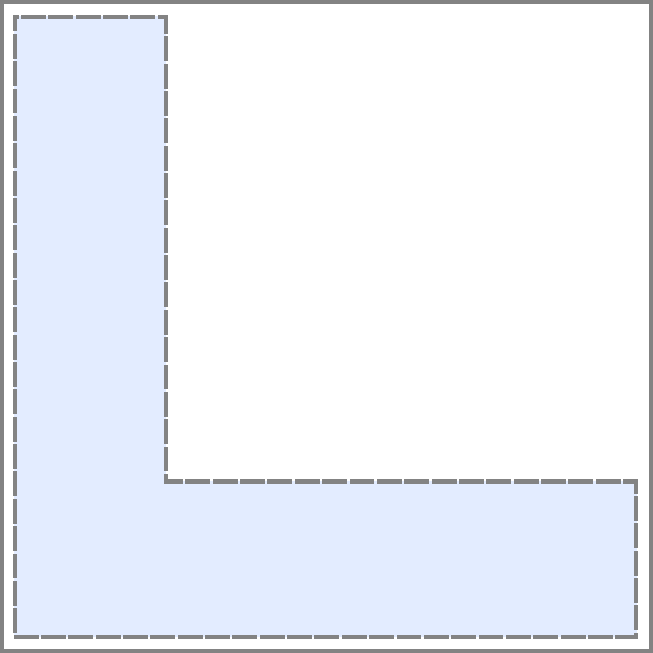
\includegraphics[width=\unitlength,page=1]{figures/ch4/extended_model_layout.pdf}}%
    \put(0.96439303,0.04406388){\color[rgb]{0.45882353,0.45882353,0.45882353}\makebox(0,0)[rt]{\lineheight{1.25}\smash{\begin{tabular}[t]{r}$k=0$\end{tabular}}}}%
    \put(0,0){\includegraphics[width=\unitlength,page=2]{figures/ch4/extended_model_layout.pdf}}%
    \put(0.96744647,0.29040942){\color[rgb]{0.45882353,0.45882353,0.45882353}\makebox(0,0)[rt]{\lineheight{1.25}\smash{\begin{tabular}[t]{r}$k=2$\end{tabular}}}}%
    \put(0,0){\includegraphics[width=\unitlength,page=3]{figures/ch4/extended_model_layout.pdf}}%
    \put(0.83910713,0.77322536){\color[rgb]{0,0,0}\transparent{0.99722999}\makebox(0,0)[t]{\lineheight{1.25}\smash{\begin{tabular}[t]{c}forest site\end{tabular}}}}%
    \put(0,0){\includegraphics[width=\unitlength,page=4]{figures/ch4/extended_model_layout.pdf}}%
    \put(0.49135778,0.43475178){\color[rgb]{0,0,0}\makebox(0,0)[t]{\lineheight{1.25}\smash{\begin{tabular}[t]{c}field site\end{tabular}}}}%
    \put(0.15604698,0.08083337){\color[rgb]{0.45882353,0.45882353,0.45882353}\makebox(0,0)[t]{\lineheight{1.25}\smash{\begin{tabular}[t]{c}field site\end{tabular}}}}%
    \put(0,0){\includegraphics[width=\unitlength,page=5]{figures/ch4/extended_model_layout.pdf}}%
    \put(0.70316853,0.28731055){\color[rgb]{0.45882353,0.45882353,0.45882353}\makebox(0,0)[rt]{\lineheight{1.25}\smash{\begin{tabular}[t]{r}$k=1$\end{tabular}}}}%
    \put(0.61707673,0.54175073){\color[rgb]{0,0,0}\makebox(0,0)[rt]{\lineheight{1.25}\smash{\begin{tabular}[t]{r}\textbf{(ii)}\end{tabular}}}}%
    \put(0.31959477,0.1993703){\color[rgb]{0,0,0}\makebox(0,0)[lt]{\lineheight{1.25}\smash{\begin{tabular}[t]{l}\textbf{(i)}\end{tabular}}}}%
    \put(0.79797428,0.92542789){\color[rgb]{0,0,0}\makebox(0,0)[lt]{\lineheight{1.25}\smash{\begin{tabular}[t]{l}\textbf{(iii)}\end{tabular}}}}%
  \end{picture}%
\endgroup%
